\chapter{Dasar Teori}
\label{chap:teori}
Bab ini berisi dasar teori dari pembangunan Aplikasi Pencarian Rute Kendaraan Umum untuk Windows Phone. Beberapa teori yang dibahas dalam bab ini  adalah Kiri API, Web Service, Menampilkan Peta, Penggunaan \textit{Global Positioning System} di Windows Phone, dan antarmuka perangkat lunak yang dibuat. 

% Windows Phone
\section{Windows Phone}
\label{sec:Windows Phone}
\hspace{0.5cm} Sub bab ini akan membahas pemrograman di Windows Phone. Pembahasan akan dimulai dengan apa itu Windows Phone dan fitur di Windows Phone yang akan digunakan dalam pembangunan perangkat lunak Pencarian Rute Kendaraan di Windows Phone. 

Windows Phone merupakan sistem operasi untuk perangkat bergerak yang dikembangkan Microsoft.\footnotemark[1] Untuk mengembangkan aplikasi Windows Phone dibutuhkan Windows Desktop 8 sebagai media pengembangan. Bahasa pemrograman yang digunakan untuk membuat perangkat lunak di Windows Phone yaitu C\#.  
%kutipan mengenai windows phone
\footnotetext[1]{\url{en.wikipedia.org/wiki/Windows_Phone}}

% SUB Mengenai Phone Control
\subsection{Phone Control}
\label{subsec:Phone Control}
\hspace{0.5cm} Phone Control merupakan blok bangunan dari antarmuka aplikasi. Windows Phone 8 menyediakan banyak set untuk hal ini dari tombol, kontrol masukan untuk mendapatkan informasi sampai ke menu. 

% SUB SUB Mengenai Tata Letak
\subsubsection{Tata Letak}
\label{subsubsec:Tata Letak}

\hspace{0.5cm} Ada 3 objek yang dipakai untuk menangani Tata Letak yaitu Grid, StackPane, dan Canvas. Perlu diperhatikan bahwa setiap halaman hanya memiliki satu Tata Letak.

\begin{itemize}
	\item Grid memposisikan elemen di baris dan kolom dari sel.
	\item StackPanel memposisikan element di jajaran horizontal atau vertical.
	\item Canvas memposiskan elemen sebagai absolut kordinat.
\end{itemize}
	
% SUB SUB Mengenai Tombol Kontrol
\subsubsection{Tombol Kontrol}
\label{subsubsec:Tombol Kontrol}
\hspace{0.5cm} Windows Phone 8 telah menyiapkan berbagai tombol yang dibutuhkan yaitu radio, check boxes, hyperlink dan repeat. Berikut tombol-tombol yang tersedia dalam bentuk kelas diagram.

\begin{figure}[h]
	\centering
		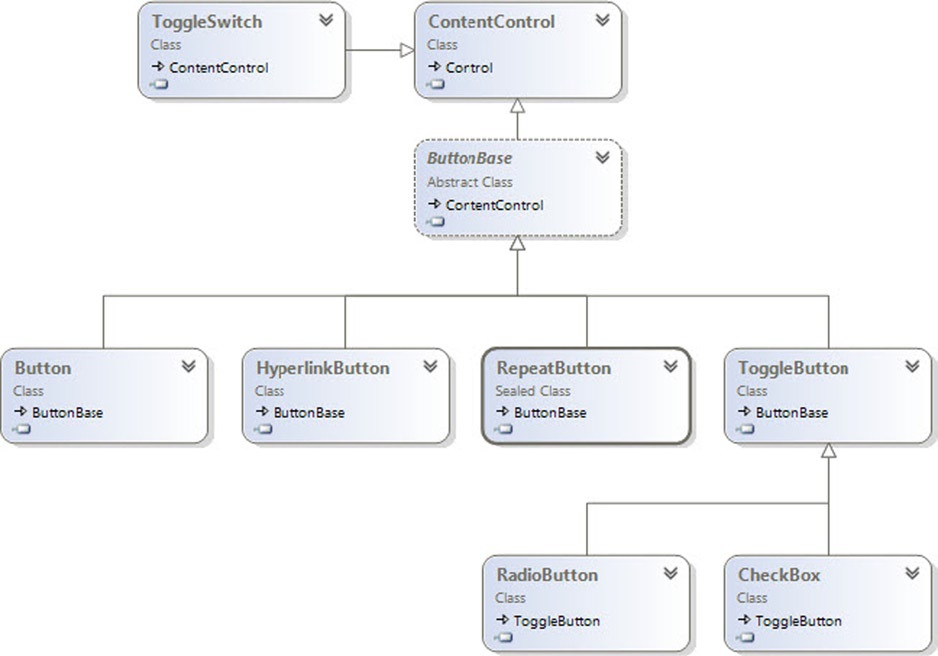
\includegraphics[scale=0.5]{Gambar/button_class_diagram.jpg}
	\caption{Kelas Diagram Button}
	\label{fig:button_class_diagram}
\end{figure}

\begin{lstlisting} [caption= Pemanggilan Search dengan Click]
	private void ClickButton_Click(object sender, RoutedEventArgs e)
	{
		SearchTask searchTask = new SearchTask();
		searchTask.SearchQuery = "Windows Phone 8";
		searchTask.Show();
	}
\end{lstlisting}

\begin{lstlisting} [caption= Perintah Pemanggilan Search]
	public class SearchCommand : ICommand
	{
		public bool CanExecute(object parameter)
		{
			return true;
		}
		public event EventHandler CanExecuteChanged;
		public void Execute(object parameter)
		{
			SearchTask searchTask = new SearchTask();
			searchTask.SearchQuery = "Windows Phone 8";
			searchTask.Show();
		}
	}
\end{lstlisting}

\begin{lstlisting} [caption= XAML Kode untuk Event Click dan Perintah]
	<Button Content="Fire Click" Click="button1_Click" />
	
	<Button Content="Fire Command" Command="{StaticResource SearchCommand}" />
\end{lstlisting}
	
% SUB SUB Mengenai Kontrol Masukan
\subsubsection{Kontrol Masukan}
\label{subsubsec:Kontrol Masukan}
\hspace{0.5cm} Semua input merupakan turunan dari kontrol, kelas yang memperkenalkan ControlTemplate yang mendefinisikan penampilan.

% SUB SUB SUB TextBox
\paragraph{TextBox}
\label{subsubsec:TextBox}
merupakan tempat masukan untuk data. Data dimasukan ketika keyboard muncul. Banyak properti yang bisa diatur dari sebuah TextBox mulai panjang maksimum hingga tata letak hingga \textit{alighment}.

\begin{lstlisting} [caption= Kode Untuk TextBox]
	<TextBox AcceptsReturn="True" TextWrapping="Wrap" Height="150"
Text="This is text that will appear on several lines. This will also handle carriage returns." />
\end{lstlisting}

\begin{figure}[h]
	\centering
		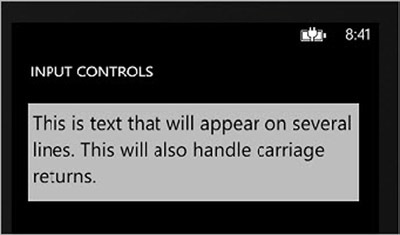
\includegraphics{Gambar/textbox.jpg}
	\caption{TextBox}
	\label{fig:textbox}
\end{figure}

% SUB SUB SUB ListPicker
\paragraph{ListPicker}
\label{subsubsec:ListPicker}
\vspace{0.5cm}
mirip dengan ComboBox untuk menampilkan beberapa item dan dapat dipilih salah satunya. Untuk tampilan ListPicker dapat ditampilkan dalam beberapa mode yaitu item yang dipilih yang ditampilkan, semua item ditampilkan di halaman baru, dan \textit{popup}.

\begin{figure}[h]
	\centering
		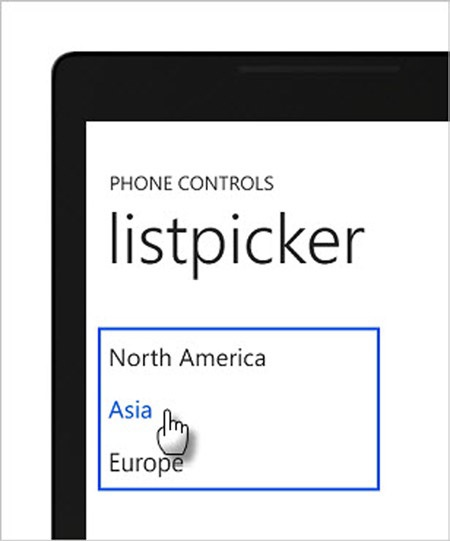
\includegraphics[scale=0.5]{Gambar/listpicker.jpg}
	\caption{Memilih dari ListPicker}
	\label{fig:listpicker}
\end{figure}

\begin{lstlisting} [caption= ListPicker di XAML]
	<toolkit:ListPicker x:Name="RegionPicker">
		<toolkit:ListPickerItem Content="North America" />
		<toolkit:ListPickerItem Content="Asia" />
		<toolkit:ListPickerItem Content="Europe" />
	</toolkit:ListPicker>
\end{lstlisting}

\begin{lstlisting} [caption= Mendefinisikan ListPicker dengan Kode]
	RegionPicker.Items.Add(new ListPickerItem()
	{
		Content = "North America",
		Tag = 123
	});
	RegionPicker.Items.Add(new ListPickerItem()
	{
		Content = "Asia",
		Tag = 456
	});
	RegionPicker.Items.Add(new ListPickerItem()
	{
		Content = "Europe",
		Tag = 789
	});
\end{lstlisting}

\begin{lstlisting} [caption= Pengambilan Data ListPicker]
	<toolkit:ListPicker x:Name="RegionPicker"
		ItemsSource="{StaticResource Regions}" >
		<toolkit:ListPicker.ItemTemplate>
			<DataTemplate>
				<StackPanel Orientation="Horizontal">
					<TextBlock Text="{Binding Id}" Margin="5"
						Style="{StaticResource PhoneTextSubtleStyle}" />
					<TextBlock Text="{Binding RegionName}" Margin="5"/>
				</StackPanel>
			</DataTemplate>
		</toolkit:ListPicker.ItemTemplate>
	</toolkit:ListPicker>
\end{lstlisting}

% SUB Mengenai Navigation
\subsection{Navigation}
\label{subsec:Navigation}
\hspace{0.5cm} Ada tiga pilihan untuk bepergian di Windows Phone: dalam halaman, antara halaman, dan URIs eksternal. Navigasi antara halman yang digunakan untuk perbedaan pandang seperti Panorama dan Pivot. Navigasi antara halaman menggunakan framework navigasi. 

% SUB SUB Navigasi Antar Halaman
\subsubsection{Navigasi Antar Halaman}
\label{subsubsec:Navigasi Antar Halaman}

\begin{figure}[h]
	\centering
		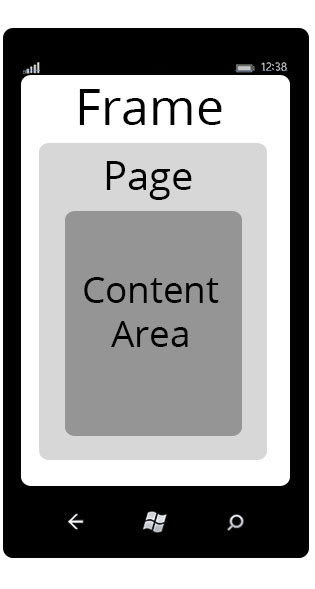
\includegraphics[scale=0.5]{Gambar/nav_hierarchy.jpg}
	\caption{Hirarki Navigasi}
	\label{fig:nav_hierarchy}
\end{figure}

% SUB SUB SUB Frame Aplikasi
\paragraph{Frame Aplikasi}
\label{subsubsec:Frame Aplikasi}
merupakan penampung terluar di hirarki kontrol untuk Windows Phone 8. Frame aplikasi ini mendukun navigasi antara halaman. Navigasi ke halaman yang lain akan menetapkan halaman yang baru sebagai frame.

\begin{lstlisting} [caption= Navigasi dengan Frame]
	private void PhoneAppFrame_Click(object sender, RoutedEventArgs e)
	{
		App.RootFrame.Navigate(new Uri("/SecondPage.xaml", UriKind.Relative));
	}
\end{lstlisting}

% SUB SUB SUB Page Aplikasi
\paragraph{Page Aplikasi}
\label{subsubsec:Page Aplikasi}
dapat dibedakan menjadi 4 yaitu OnFragmentNavigation, OnNavigationForm, OnNavigatedFrom, dan OnNavigatedTo. Berikut penjelasan dan contoh kodenya:

\begin{itemize}
	\item OnFragmentNavigation: Fragment merupakan bagian URI yang diikuti tanda "\#" dan dipakai untuk memberikan detail antar halaman. Pada kode dibawah menunjukan navigasi ke halaman dua sambil memberikan fragment string "detail".
	
	\begin{lstlisting} [caption= Halaman Utama melewati fragment ke lamana kedua]
		private void PageFragment_Click(object sender, RoutedEventArgs e)
		{
			App.RootFrame.Navigate(new Uri("/SecondPage.xaml#detail", UriKind.Relative));
		}
	\end{lstlisting}
	
	\begin{lstlisting} [caption= Halaman Utama melewati fragment ke lamana kedua]
		protected override void OnFragmentNavigation(FragmentNavigationEventArgs e)
		{
			// displays "Fragment: Detail"
			MessageBox.Show("Fragment: " + e.Fragment);
			base.OnFragmentNavigation(e);
		}
	\end{lstlisting}

	\item OnNavigationForm: Dipakai untuk langkah pencegahan saat pengguna akan meninggalkan halaman.	
	\begin{lstlisting} [caption= Sebelum Navigasi]
		protected override void OnNavigatingFrom(NavigatingCancelEventArgs e)
		{
		e.Cancel = MessageBox.Show("You have unsaved data, do you want to exit?", "Unsaved data",
		MessageBoxButton.OKCancel) == MessageBoxResult.Cancel;
		base.OnNavigatingFrom(e);
		}
	\end{lstlisting}
	
	\item OnNavigatedFrom: Metode dipanggil ketika halaman sudah tidak aktif lagi. NavigationEventArgs merupakan halaman yang dituju. Hal ini untuk mendukung pengiriman data dari halaman yang ditinggalkan dan mengirimnya ke halaman yang mau ditampilkan.
	\begin{lstlisting} [caption= Setelah Navigasi ]
		// Navigated from "SecondPage" back to "MainPage"
		protected override void OnNavigatedFrom(NavigationEventArgs e)
		{
			MainPage mainPage = e.Content as MainPage;
			if (mainPage != null)
				mainPage.StatusText.Text = "A message from SecondPage OnNavigatedFrom";
			base.OnNavigatedFrom(e);
		}
	\end{lstlisting}
	
	\item OnNavigatedTo: Netode dipanggil ketika halaman sudah aktif.
	\begin{lstlisting} [caption= Navigasi ke Halaman Berikutnya]
		protected override void OnNavigatedTo(NavigationEventArgs e)
		{
			MessageBox.Show("NavigatedTo: " + e.Uri);
			base.OnNavigatedTo(e);
		}
	\end{lstlisting}
\end{itemize}

% SUB SUB SUB Layanan Navigasi
\paragraph{Layanan Navigasi}
\label{subsubsec:Layanan Navigasi}
merupakan layanan untuk memantau riwayat navigasi, menyediakan metode navigasi, dan event. Layanan ini juga memungkinkan perpindahan navigasi sesuai riwayat menggunakan GoBack() dan GoForward(). Berikut contoh metodenya.

\begin{lstlisting} [caption= Metode Layanan Navigasi ]
		this.NavigationService.Navigate(new Uri("/SecondPage.xaml", UriKind.Relative));
\end{lstlisting}

% SUB SUB Navigasi ke URIs Eksternal
\subsubsection{Navigasi ke URIs Eksternal}
\label{subsubsec:Navigasi ke URIs Eksternal}

\begin{lstlisting} [caption= Navigasi dengan Web Browser]
	WebBrowserTask webBrowserTask = new WebBrowserTask();
	webBrowserTask.Uri = new Uri("http://www.falafel.com");
	webBrowserTask.Show();
\end{lstlisting}

% SUB Mengenai Lifecycle
\subsection{Lifecycle Windows Phone}
\label{subsec:Lifecycle Windows Phone}

\begin{itemize}
	\item Running : Aplikasi sedang berada di bagian depan. Hanya satu aplikasi yang diijinkan berada di depan pada satu waktu.
	\item Dormant : Aplikasi tidak berada di bagian depan, tetapi sistem operasi tidak membutuhkan sumber daya(dalam hal ini memori). Pada tahap ini objek aplikasi masih berada di memori, jadi pada tahap Dormant aplikasi dapat secara otomatis diaktifkan kembali. Tetapi jika sistem operasi  membutuhkan sumbe daya maka aplikasi akan menjadi \textit{tombstoned} dan dihancurkan. 
	\item Tombstoned : Aplikasi akan dihancurkan dan objek aplikasi akan dihapus dari memori. Ketika aplikasi diaktivasi pengguna akan ditempatkan kembali di halaman yang ditinggalkan sebelumnya, tetapi objek harus di kembalikan dari keadaan sebelumnya.
\end{itemize}

% SUB SUB Penyimpanan dan Pengembalian Keadaan Aplikasi
\subsubsection{Penyimpanan dan Pengembalian Keadaan Aplikasi}
\label{subsubsec:Penyimpanan dan Pengembalian Keadaan Aplikasi}

\begin{lstlisting} [caption= App.xaml]
	<Application.ApplicationLifetimeObjects>
		<!--Required object that handles lifetime events for the application-->
		<shell:PhoneApplicationService
			Launching="Application_Launching" Closing="Application_Closing"
			Activated="Application_Activated" Deactivated="Application_Deactivated"/>
	</Application.ApplicationLifetimeObjects>
\end{lstlisting}

\begin{lstlisting} [caption= Appp.xaml.cs]
	// Code to execute when the application is launching (eg, from Start)
	// This code will not execute when the application is reactivated
	private void Application_Launching(object sender, LaunchingEventArgs e)
	{
	}
	// Code to execute when the application is activated (brought to foreground)
	// This code will not execute when the application is first launched
	private void Application_Activated(object sender, ActivatedEventArgs e)
	{
	}
	// Code to execute when the application is deactivated (sent to background)
	// This code will not execute when the application is closing
	private void Application_Deactivated(object sender, DeactivatedEventArgs e)
	{
	}
	// Code to execute when the application is closing (eg, user hit Back)
	// This code will not execute when the application is deactivated
	private void Application_Closing(object sender, ClosingEventArgs e)
	{
	}
\end{lstlisting}

\begin{lstlisting} [caption= Penanganan terhadap pengaktifan dan penonaktifan kejadian]
	public class MyObject
	{
	public DateTime LastUpdate { get; set; }
	}
	//...
	public MyObject MyObject { get; set; }
	
	private void Application_Activated(object sender, ActivatedEventArgs e)
	{
		DateTime lastUpdate =
		(DateTime)PhoneApplicationService.Current.State["LastUpdate"];
		Debug.WriteLine("Application_Activated: LastUpdate=" + lastUpdate.ToLongTimeString());
	}
	private void Application_Deactivated(object sender, DeactivatedEventArgs e)
	{
		Debug.WriteLine("Application_Deactivated: Saving LastUpdate to application state");
		PhoneApplicationService.Current.State["LastUpdate"] = DateTime.Now;
	}
\end{lstlisting}

% SUB Peta di Windows Phone
\subsection{Peta di Windows Phone}
\label{subsec:Peta di Windows Phone}
\hspace{0.5cm} Peta untuk Windows Phone adalah Here Maps. Here Maps yang akan menampilkan lokasi dan melakukan penelusuran. Pada Sub Bab ini akan dibahas mengenai penambahan peta pada aplikasi, mendapatkan lokasi, petunjuk arah dan Pushpins.

% SUB SUB Mengenai Penambahan Maps Ke Aplikasi
\subsubsection{Penambahan Maps Ke Aplikasi}
\label{subsubsec:Penambahan Maps Ke Aplikasi}
\hspace{0.5cm} Ada dua cara untuk menambahkan peta ke aplikasi yang pertama dengan menjalankan MapTask dan yang kedua dengan ppenambahan ID\_CAP\_MAP ke \textbackslash properties\textbackslash WMAppManifest.xml. Contoh dibawah adalah dengan MapTask yang memenggil metode Show() untuk memunculkan peta.

\begin{lstlisting} [caption= code pemanggilan maps]
	private void MapClick(object sender, EventArgs e)
	{
		var task = new MapsTask();
		var goldenGateBridge = new GeoCoordinate(37.8085880, -122.4770175);
		task.Center = goldenGateBridge;
		task.ZoomLevel = 9;
		task.SearchTerm = "Golden Gate Bridge";
		task.Show();
	}
\end{lstlisting}

\begin{lstlisting} [caption= penambahan Map Element menggunakan Map Control]
	<Grid x:Name="LayoutRoot" Background="Transparent">
		<Controls:Map x:Name="WorldMap" />
	</Grid>
\end{lstlisting}

% SUB SUB Mengenai Posisi Pada Peta
\subsubsection{Posisi Pada Peta}
\label{subsubsec:Posisi Pada Peta}
\hspace{0.5cm} Ketika memulai membuka peta maka akan menampilkan seluruh dunia dan pengguna harus melakukan \textit{pinch-and-zoom} untuk melihat titk tertentu. Agar dapat memudahkan pengguna dalam memilih titik tertentu secara otomatis maka dapat menggunakan metode SetView\(\). Pada Listing dibawah dapat dilihat bahwa SetView\(\) memiliki 2 parameter. Parameter pertama menyatakan tempat dengan GeoCordinate yang mendefinisikan pusat pandangan. Selanjutnya parameter ke 2 merupakan zoomLevel ( 1 = zoomed out, 20 = zoomed in). 

\begin{lstlisting} [caption= Posisi Pada Peta]
	GeoCoordinate GoldenGateBridge = new GeoCoordinate(37.8085880, -122.4770175);
	SanFranciscoMap.SetView(GoldenGateBridge, 15);
\end{lstlisting}

% SUB SUB Penambahan Pushpins ke Peta
\subsubsection{Penambahan Pushpins ke Peta}
\label{subsubsec:Penambahan Pushpins ke Peta}

\hspace{0.5cm} Peta tidak mendukung langsung cara untuk mengikat data ke MapLayer dan MapOverlay. Untungnya di Windows Phone memiliki Windows Phone 8 Toolkit yang memiliki set objek yang dapat digunakan sebagai jembatan mengikat data ke MapLayer dan MapOverlay.

\begin{lstlisting} [caption= Berikut contoh Tookkit Pushpin dengan elemen-element yang di tulisa manual]
	<Controls:Map>
		<Toolkit:MapExtensions.Children>
			<Toolkit:Pushpin Content="London" GeoCoordinate="51.499493,-0.124753" />
		</Toolkit:MapExtensions.Children>
	</Controls:Map>
\end{lstlisting}

\hspace{0.5cm} Gambar dibawah merupakan keluaran di peta. Label "London" merupkan bawaan Windows Phone 8 pushpin.

\begin{figure}[!h]
	\centering
		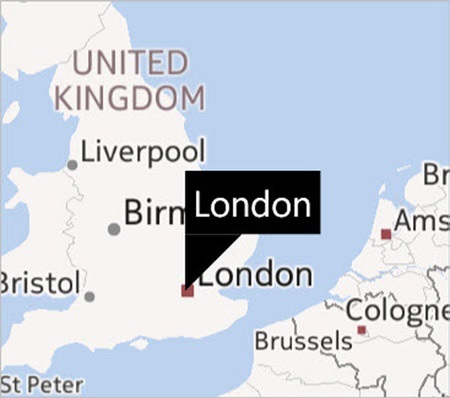
\includegraphics[scale=0.5]{Gambar/toolkit_pushpin.jpg}
	\caption{Keluaran Toolkit Pushpin pada Peta}
	\label{fig:toolkit_pushpin}
\end{figure}

\hspace{0.5cm} Selain menetapkan Pushpin secara langsung  di MapExtensions, dapat pula diletakan MapItemsControl. Pushpin akan berpindah ke ItemTemplate dan ItemSource akan ditugaskan ViewModel.

\begin{lstlisting} [caption= Berikut contoh Tookkit Pushpin dengan elemen-element yang di tulisa manual]
	<Controls:Map x:Name="WorldMap" >
		<Toolkit:MapExtensions.Children>
			<Toolkit:MapItemsControl ItemTemplate="{StaticResource MapItemTemplate}" ItemsSource="{Binding Source={StaticResource LocationViewModel}, Path=Locations}" />
		</Toolkit:MapExtensions.Children>
	</Controls:Map>
\end{lstlisting}

\begin{lstlisting} [caption= View Model]
	public class Location
	{
		public string Title { get; set; }
		[TypeConverter(typeof(GeoCoordinateConverter))]
		public GeoCoordinate GeoCoordinate { get; set; }
	}
	
	public class LocationViewModel
	{
		public ObservableCollection<Location> Locations { get; set; }
		public LocationViewModel()
		{
			Locations = new ObservableCollection<Location>();
		}
	}
\end{lstlisting}

\begin{lstlisting} [caption= Deklarasi View Model]
	<phone:PhoneApplicationPage.Resources>
		<vm:LocationViewModel x:Key="LocationViewModel" >
			<vm:LocationViewModel.Locations>
				<vm:Location Title="London" GeoCoordinate="51.499493,-0.124753" />
				<vm:Location Title="Paris" GeoCoordinate="48.858222,2.2945" />
				<vm:Location Title="Rome" GeoCoordinate="41.890268,12.492315" />
			</vm:LocationViewModel.Locations>
		</vm:LocationViewModel>
		<DataTemplate x:Name="MapItemTemplate">
			<Toolkit:Pushpin GeoCoordinate="{Binding GeoCoordinate}" Content="{Binding Title}" />
		</DataTemplate>
	</phone:PhoneApplicationPage.Resources>
\end{lstlisting}

% SUB SUB Mendapatkan Posisi Pengguna
\subsubsection{Mendapatkan Posisi Pengguna}
\label{subsubsec:Mendapatkan Posisi Pengguna}
\hspace{0.5cm} Di Windows Phone 8 telah ada GeoCoordinate yang dapat digunakan untuk mengetahui posisi pengguna. Geolocator dari Windows.Devices.Geolocation akan mengembalikan posisi saat ini. Tetapi untuk menggunakan Geolocator, penulis perlu menghidupkan ID\_CAP\_LOCATION di \textbackslash properties\textbackslash WMAppManifest.xml. 

\hspace{0.5cm} Contoh kode dari penggunaan menggunakan XAML didefinisikan pada listing dibawah. UserLocationMarker di MapExtensions Children.UserLocationMarker merupakan Toolkit objek Windows Phone 8. Visibilitas UserLocationMarker di set "collapsed" agar penanda tetap berada di tempat sampai ada perubahan lokasi dan siap ditampilkan.

\begin{lstlisting} [caption= Map dan UserLocationMarker XAML]
	Grid x:Name="ContentPanel" Grid.Row="1" Margin="12,0,12,0">
		<Controls:Map x:Name="WorldMap">
			<Toolkit:MapExtensions.Children>
				<Toolkit:UserLocationMarker x:Name="locationMarker" Visibility="Collapsed" />
			</Toolkit:MapExtensions.Children>
		</Controls:Map>
	</Grid>
\end{lstlisting}

\hspace{0.5cm} Listing Dibawah akan mendemokan bagaimana GeoLocator mendapatkan posisi terkini. Contoh dari metode menggunakan \textit{event} click. setelah itu dipanggil GetGeopositionAsync() yang akan mengembalikan objek GeoPosition object.GetGeopositionAsync yang sip menunggu, jadi tambahkan async untuk pemanggilan metode dan kata kunci await untuk mendapatkan nilai kembalian. Geoposition mengandung kordinat yang tidak kompatibel dengan GeoCoordinate() yang dipakai untuk map. Untungnya toolkit menyediakan metode ToGeoCoordinate() untuk menerjemahkan ke GeoCoordinate secara otomatis. Kode dibawah juga menjadi referensi pemakaian UserLocationMarker, makes it visible, dan di set menjadi GeoCordinate baru. Terakhir, metode Map SetView() dipanggil untuk menjadi pusat dari posisi yang baru.

\begin{lstlisting} [caption= Setting ulang Geolocator]
	private Geolocator _locator;
	protected override void OnNavigatedTo(NavigationEventArgs e)
	{
		base.OnNavigatedTo(e);
		_locator = new Geolocator()
		{
			// set either ReportInterval (milliseconds) or MovementThreshold (meters)
			ReportInterval = 5000,
			//DesiredAccuracy = PositionAccuracy.High
			DesiredAccuracyInMeters = 1
		};
		_locator.PositionChanged += _locator_PositionChanged;
	}
\end{lstlisting}

\begin{lstlisting} [caption= Melepas Geolocator yang dapat dipakai untuk melindungi sumber daya]
	protected override void OnNavigatedFrom(NavigationEventArgs e)
	{
		_locator.PositionChanged -= _locator_PositionChanged;
		_locator = null;
		base.OnNavigatedFrom(e);
	}
\end{lstlisting}

\begin{lstlisting} [caption= Menangani Perubahan Posisi]
	void _locator_PositionChanged(Geolocator sender, PositionChangedEventArgs args)
	{
		this.Dispatcher.BeginInvoke(() =>
			{
				var geoCoordinate = args.Position.Coordinate.ToGeoCoordinate();
				var locationMarker = this.FindName("locationMarker") as UserLocationMarker;
				if (locationMarker != null)
				{
				locationMarker.Visibility = System.Windows.Visibility.Visible;
				locationMarker.GeoCoordinate = geoCoordinate;
				WorldMap.SetView(geoCoordinate, 15);
				}
			});
	}
\end{lstlisting}

\begin{lstlisting} [caption= Menangani Perubahan Status]
	void _locator_StatusChanged(Geolocator sender, StatusChangedEventArgs args)
	{
		this.Dispatcher.BeginInvoke(() =>
		{
			var textBlock = this.FindName("StatusText") as TextBlock;
			textBlock.Text = "Status: " + args.Status.ToString();
		});
	}
\end{lstlisting}

Berikut nilai yang mungkin dari Status Posisi:
\begin{itemize}
	\item \textit{Ready} : Jika lokasi tersedia.
	\item \textit{Initializing} : Status jika penangkap GPS belum memiliki cukup satelit untuk mendapatkan posisi yang akurat. 
	\item \textit{NoData} : Data lokasi belum tersedia. Status ini muncul jika aplikasi sedang mamanggil GetGeopositionAsync atau register.
	\item \textit{Disable} : Status mengindikasikan tidak diperbolehkannya pengaksesan lokasi.
	\item \textit{NotInitialized} : Data lokasi belum tersedia. Status ini muncul jika aplikasi belum mamanggil GetGeopositionAsync atau register.
	\item \textit{NotAvailable} : Jika Windows sensor dan lokasi tidak tersedia.
\end{itemize}

% SUB SUB Arah
\subsubsection{Arah}
\label{subsubsec:Arah}
\hspace{0.5cm} Penambahan langkah demi langkah arah rute di aplikasi di Windows Phone 8 mudah dilakukan. Untuk memunculkan arah cukup memiliki titik awal dan titik akhir. Pada listing dibawah mendemontrasikan pengarahan di map antara 2 titik. Untuk titik awal dan akhir perlu label lokasi dengan objek LabeledMapLocation. Selanjutnya setelah menetapkan dua objek pada MapsDirectionsTask lalu panggil metode show() dan arah dari titk awal ke titik akhir akan muncul di peta.    

\begin{lstlisting} [caption= Penggunaan Arah pada Map]
	var wharf = new LabeledMapLocation()
	{
		Label = "Wharf",
		Location = new GeoCoordinate(36.96252, -122.023372)
	};
	var park = new LabeledMapLocation()
	{
		Label = "Lighthouse Park",
		Location = new GeoCoordinate(36.95172, -122.026783)
	};
	var task = new MapsDirectionsTask() { Start = wharf, End = park };
	task.Show();
\end{lstlisting}

\hspace{0.5cm} Meskipun Map bisa menggambar rute secara otomatis ada satu cara lagi untuk menambahkan objek tute pada Map yaitu menggunakan RouteQuery. Pertama yang harus didefinisikan pada RouteQuery yaitu GeoCoordinate yang harus dikunjungi. Pada listing dibawah dapat dilihat 3 GeoCoordinate dijadikan Waypoints di RouteQuery yang baru. RouteOptimization di pakai untuk meminimalisir jarak dan TraveMode di setel Driving. 

\begin{lstlisting} [caption= Mengatur Ulang Rute Query]
	var wharf = new GeoCoordinate(36.96252, -122.023372);
	var park = new GeoCoordinate(36.95172, -122.026783);
	var lagoon = new GeoCoordinate(36.963365, -122.031932);
	var routeQuery = new RouteQuery()
	{
		Waypoints = new List<GeoCoordinate>() { wharf, park, lagoon },
		RouteOptimization = RouteOptimization.MinimizeDistance,
		TravelMode = TravelMode.Driving
	};
	routeQuery.QueryCompleted += routeQuery_QueryCompleted;
	routeQuery.QueryAsync();
\end{lstlisting}

\hspace{0.5cm} Untuk melakukan handle terhadap QueryCompleted, pertama harus di periksa apakah terdapat kesalahan. Kembaliannya adalah objek rute. Lalu jadikan MapRoute konstruktor. MapRoute menambahkan visualisasi garis pada peta. Contoh implementasinya dapat dilihat di listing dibawah.

\begin{lstlisting} [caption= Melakukan Handle Terhadap QueryCompleted]
	void routeQuery_QueryCompleted(object sender, QueryCompletedEventArgs<Route> e)
	{
		if (e.Error == null)
		{
			this.WorldMap.AddRoute(new MapRoute( e.Result));
			this.WorldMap.SetView(e.Result.BoundingBox);
		}
	}
\end{lstlisting}

\begin{lstlisting} [caption= Melakukan Perubahan Warna Rute di Map]
	var mapRoute = new MapRoute(e.Result)
	{
		Color = Colors.Red,
		RouteViewKind = RouteViewKind.UserDefined
	};
	this.WorldMap.AddRoute(mapRoute)
\end{lstlisting}

\begin{lstlisting} [caption= Menampilkan Arah dalam Bentuk List]
	var sb = new StringBuilder();
	var i = 0;
	sb.AppendFormat("Estimated time: {0} minutes\n",
		e.Result.EstimatedDuration.TotalMinutes.ToString());
	foreach (var leg in e.Result.Legs)
	{
		foreach (var maneuver in leg.Maneuvers)
		{
			sb.AppendFormat("{0}. {1}: {2}\n",++i, maneuver.InstructionKind.ToString(), maneuver.InstructionText);
		}
	}
	MessageBox.Show(sb.ToString());
\end{lstlisting}

% SUB Memanfaatkan Sumber Data
\subsection{Memanfaatkan Sumber Data}
\label{subsec:Memanfaatkan Sumber Data}

% SUB SUB Serializing Object
\subsubsection{Serializing Object}
\label{subsubsec:Serializing Object}
\hspace{0.5cm} \textit{Serialization} disini merupakan proses mentransformasikan objek ke format yang bisa dengan mudah dikirim melewati jaringan atau disimpan di database. Formatnya disini berupa string yang direpresentasikan sebagai objek di XML atau JSON(Javascript Object Notation). Ada beberapa objek yang dapat melakukan serialisasi, tetapi yang akan dibahas penulis disini hanya serialisasi JSON. 

\hspace{0.5cm} Banyak \textit{web service} yang mengembalikan data dalam format JSON. JSON memiliki struktur yang mudah dipahami dimana kurung kurawal mengindikasikan objek, kurung siku berarti array, dan properti berupa nama dan nilai pasangan yang dipisahkan oleh titik dua. JSON format memiliki ukuran data yang kecil dan baik untuk penggunaan perangkat bergerak. Untuk contoh format JSON dapat dilihat di bagian Kiri API pada Bab 2 ini karena Kiri API menggunakan format JSON. Serialisasi menggunakan DataContractJsonSerializer membuat serialisasi mudah untuk menerjemahkan form String JSON ke objek yang dapat langsung digunakan. DataContractJsonSerializer memakai WriteObject() untuk serialisasi and ReadObject() untuk de-serialisasi.

% SUB SUB Memanfaatkan Sumber Data Web
\subsubsection{Memanfaatkan Sumber Data Web}
\label{subsubsec:Memanfaatkan Sumber Data Web}

\begin{lstlisting} [caption= Pembentuk getPublicPhotos Url pada flicker]
	private const string BaseUrl = "http://ycpi.api.flickr.com/services/rest/";
	private const string QueryStrings =
	"?method={0}&api_key={1}&user_id={2}&format=json&nojsoncallback=1";
	private const string FlickrMethod = "flickr.people.getPublicPhotos";
	private const string YourApiKey = "<replace with api key here>";
	private const string LibraryOfCongressKey = "8623220@N02";
	private string FlickrPhotosUrl = BaseUrl +
	String.Format(QueryStrings, FlickrMethod, YourApiKey, LibraryOfCongressKey);
\end{lstlisting}

\begin{lstlisting} [caption= Contoh JSON String dari flickr API]
	{
		"photos":{
			"page":1,
			"pages":193,
			"perpage":100,
			"total":"19222",
			"photo":[
				{
					"id":"9319237625",
					"owner":"8623220@N02",
					"secret":"e0d73d680b",
					"server":"5537",
					"farm":6,. . .
\end{lstlisting}

\hspace{0.5cm} Selanjutnya untuk menerjemahkan JSON ke C\# bisa lewat web sites json2csharp.com. Menuju ke json2csharp.com lalu paste JSON di text box yang ada dan click Generate. Selanjutnya buat class berekstensi .cs lalu paste  text C\# yang telah di generate. 

\begin{lstlisting} [caption= Contoh JSON String dari flickr API]
	using System.Collections.Generic;
	
	namespace ConsumingXML.Classes
	{
		public class Photo
		{
			public string id { get; set; }
			public string owner { get; set; }
			public string secret { get; set; }
			public string server { get; set; }
			public int farm { get; set; }
			public string title { get; set; }
			public int ispublic { get; set; }
			public int isfriend { get; set; }
			public int isfamily { get; set; }
		}
		public class Photos
		{
			public int page { get; set; }
			public int pages { get; set; }
			public int perpage { get; set; }
			public string total { get; set; }
			public List<Photo> photo { get; set; }
		}
		public class RootObject
		{
			public Photos photos { get; set; }
			public string stat { get; set; }
		}
	}
\end{lstlisting}

\begin{lstlisting} [caption= Mengembalikan daftar FlickrPhoto]
	private static List<FlickrPhoto> GetFlickrPhotos(string json)
	{
	const string baseUrl =
	"http://farm{0}.staticflickr.com/{1}/{2}_{3}_s.jpg";
	List<FlickrPhoto> FlickrPhotos = null;
	var serializer = new DataContractJsonSerializer(typeof(RootObject));
	using (var stream = new MemoryStream(Encoding.UTF8.GetBytes(json)))
	{
	var root = serializer.ReadObject(stream) as RootObject;
	FlickrPhotos = (from photo in root.photos.photo
	select new FlickrPhoto
	{
	Title = photo.title,
	Uri = new Uri(String.Format(baseUrl,
	photo.farm, photo.server, photo.id, photo.secret))
	}).ToList();
	}
	return FlickrPhotos;
	}
\end{lstlisting}

\begin{lstlisting} [caption= Menggunakan WebClient untuk mendownload String]
	private void UseWebClient()
	{
	var uri = new Uri(FlickrPhotosUrl);
	var client = new WebClient();
	client.DownloadStringCompleted += (sender, e) =>
	{
	var photos = GetFlickrPhotos(e.Result);
	Dispatcher.BeginInvoke(() =>
	{
	FlickrListBox.DataContext = photos;
	});
	};
	client.DownloadStringAsync(uri);
}
\end{lstlisting}

\begin{lstlisting} [caption= XAML untuk halaman]
	<Grid x:Name="LayoutRoot" >
		<ListBox x:Name="FlickrListBox" ItemsSource="{Binding}">
			<ListBox.ItemTemplate>
				<DataTemplate>
					<StackPanel Orientation="Horizontal">
						<Image Stretch="UniformToFill" Width="100" Height="100" Source="{Binding Uri}" />
						<TextBlock Grid.Column="1" Margin="10,0,0,0" Text="{Binding Title}" HorizontalAlignment="Stretch" />
					</StackPanel>
				</DataTemplate>
			</ListBox.ItemTemplate>
		</ListBox>
	</Grid>
\end{lstlisting}

%Kiri API
\section{Kiri API}
\label{sec:Kiri API}
\hspace{0.5cm} Sub bab ini akan membahas Dokumentasi dari Kiri API. Pembahasan dimulai dengan pengantar dari Kiri API dan \textit{Web Service}.

% SUB Pengantar Kiri API
\subsection{Pengantar Kiri API}
\label{subsec:Pengantar Kiri API}
\hspace{0.5cm} Pemanfaatan Kiri API adalah menggunakan \textit{Web Service}. Hal ini memungkinkan pengaksesan dimana saja dengan menggunakan koneksi internet. Pemanfaatan Kiri API cukup dengan melakuan \textit{request} dengan parameter dan Kiri akan mengembalikan hasil dalam format JSON. Untuk setiap \textit{request} membutuhkan \textit{API key} yang didapat dengan mendaftar\footnotemark[2]. 
%kutipan mengenai kiri
\footnotetext[2]{\url{https://bitbucket.org/projectkiri/kiri_api/wiki/KIRI API v2 Documentation}}

% SUB Routing Web Service
\subsection{Routing Web Service}
\label{subsec:Routing Web Service}
\hspace{0.5cm} Routing Web Service merupakan Kiri API yang digunakan untuk mendapatkan langkah perjalanan dari lokasi asal ke lokasi tujuan.

Berikut parameter \textit{request} yang diperlukan berikut penjelasanya:

\begin{tabular}{ |l| |l| |l| }
	\hline
  version & 2 & \vtop{\hbox{\strut Memberitahukan bahwa layanan yang dipakai} \hbox{\strut adalah protokol veris 2}} \\ \hline
  mode & "findroute" & mengintruksikan layanan untuk mencari rute \\ \hline
  locale & "en" or "id" & bahasa yang digunakan untuk balasan \\ \hline
	start & lat,lng (both are decimal values) & titk awal \textit{Latitude} dan \textit{longitude} \\ \hline
  finish & lat,lng (both are decimal values) & titik akhir \textit{Latitude} dan \textit{longitude}  \\ \hline
  presentation & "mobile" or "desktop" & \vtop{\hbox{\strut Menentukan tipe prensentasi untuk keluaran.}\hbox{\strut Contoh, jika tipe presentasi "mobile", }\hbox{\strut maka link "tel:" akan ditambahkan di hasil.}} \\ \hline
	apikey & 16-digit hexadecimals & API key yang digunakan \\ \hline
	\hline
\end{tabular}

\vspace{5mm}
Berikut format Kiri API \textit{responds}:

\begin{lstlisting} [caption= code \textit{respond} pencarian rute]
{ 
    "status": "ok" or "error" 
    "routingresults": [ 
        {
            "steps": [
                [
                    "walk" or "none" or others,
                    "walk" or vehicle_id or "none",
                    ["lat_1,lon_1", "lan_2,lon_2", ... "lat_n,lon_n"],
                    "human readable description, dependant on locale",
                    URL for ticket booking or null (future)
                ],
                [
                    "walk" or "none" or others,
                    "walk" or vehicle_id or "none",
                    ["lat_1,lon_1", "lan_2,lon_2", ... "lat_n,lon_n"],
                    "human readable description, dependant on locale",
                    URL for ticket booking or null (future)
                ]
            ],
            "traveltime": any text string, null if and only if route is not found.
        } ,
        {
            "steps": [ ... ],
            "traveltime": "..."
        } ,
        {
            "steps": [ ... ],
            "traveltime": "..."
        } ,
        ...     
    ]
}
\end{lstlisting}
Berikut maksud dari listing 2.1:
\hspace{0.5cm} Ketika pencarian rute sukses dilakukan maka status akan memberitahukan "ok" seperti di baris 2. Selanjutnya setiap langkah dari posisi awal ke posisi tujuan akan ditampung di array dari langkah. Berikut keterangan dari setiap array tersebut: 

\begin{itemize}
	\item Index ke 0 atau baris 7 pada listing 2.1 dapat berisi "walk" atau "none" atau "others". Artinya  jika "walk" berarti berjalan kaki, "none" jika rute tidak ditemukan dan "others" berarti menggunakan kendaran.
	\item Index ke 1 atau baris 8 pada listing 2.1 merupakan detail dari index 0. Artinya jika index 0 "walk" berarti index 1 harus "walk", "none" berarti index 1 harus "none" dan selain itu menyatakan id kendaraan yang mana bisa dipakai untuk ditampilkan gambarnya.
	\item Index ke 2 atau baris 9 pada listing 2.1 adalah array string yang berisi jalur dalam format "lat,lon". Maksud dari "lat,lon" disini adalah titik permulaan dan titik selesai.
	\item Index ke 3 atau bari 10 pada listing 2.1 merupakan berisi bentuk yang akan ditampilkan kepada pengguna. Informasi yang disampaikan dapat berupa:
		\begin{itemize}
			\item \%fromicon = untuk menunjukan ikon "from". Biasanya untuk mode presentasi di perangkat bergerak.
			\item \%toicon = untuk menunjukan ikon "to". Biasanya untuk mode presentasi di perangkat bergerak. 
		\end{itemize}
	\item Index ke 4 atau bari 11 pada listing 2.1 berisi URL untuk pemesanan tiket jika tersedia. Jika tidak tersedia akan bernilai null.
\end{itemize}
 	 	
% SUB Web Service Pencarian Lokasi
\subsection{Web Service Pencarian Lokasi}
\label{subsec:Pencarian Lokasi Service}
\hspace{0.5cm} Merupakan Kiri API yang digunakan untuk mencari lokasi beserta kordinat \textit{latitude} dan \textit{longitude}

Berikut parameter \textit{request} yang diperlukan berikut penjelasanya:

\begin{tabular}{ |l| |l| |l| }
	\hline
  version & 2 & \vtop{\hbox{\strut Memberitahukan bahwa layanan yang dipakai} \hbox{\strut adalah protokol veris 2}} \\ \hline
  mode & "searchplace" & mengintruksikan layanan untuk mencari tempat \\ \hline
  region & "cgk" or "bdo" or "sub" & kota yang akan dicari tempatnya \\ \hline
	querystring & \vtop{\hbox{\strut text apa saja dengan minimum} \hbox{\strut text satu karakter}} & \vtop{\hbox{\strut query string yang akan dicari menggunakan}  \hbox{\strut layanan ini}} \\ \hline
	apikey & 16-digit hexadecimals & API key yang digunakan \\ \hline
	\hline
\end{tabular}

\vspace{5mm}
Berikut format Kiri API \textit{responds}:

\begin{lstlisting} [caption= code \textit{respond} pencarian lokasi]
{
    "status": "ok" or "error"
    "searchresult": [
        {
            "placename": "place name"
            "location": "lat,lon"
        },
        {
            "placename": "place name"
            "location": "lat,lon"
        },
        ...
    ]
    "attributions": [
        "attribution_1", "attribution_2", ...
    ]
}
\end{lstlisting}
Berikut maksud dari listing 2.2:
\hspace{0.5cm} Ketika pencarian lokasi sukses dilakukan maka status akan memberitahukan "ok" seperti di baris 2. Selanjutnya akan ditampilkan hasil dari lokasi yang ada beserta atributnya. Berikut keterangan dari format dari pencarian lokasi:
\begin{itemize}
	\item Searchresult (pada bari 4 sampai 7, 8 sampai 11, dan seterusnya) berisi array dari tempat:
	\begin{itemize}
		\item placename: nama tempat.
		\item location: latitude dan longitude dari tempat.
	\end{itemize}
	\item Attributions berisi array string yang berisikan atribut tambahan untuk dimunculkan.
\end{itemize}	

% SUB Web Service Memilih Transportasi Terdekat
\subsection{Web Service Menemukan Transportasi Terdekat}
\label{subsec:Service Menemukan Transportasi Terdekat}
\hspace{0.5cm} Merupakan Kiri API yang digunakan untuk menemukan rute transportasi terdekat sesuai titik yang diinginkan pengguna.

Berikut parameter \textit{request} yang diperlukan berikut penjelasanya:

\begin{tabular}{ |l| |l| |l| }
	\hline
  version & 2 & \vtop{\hbox{\strut Memberitahukan bahwa layanan yang dipakai} \hbox{\strut adalah protokol veris 2}} \\ \hline
  mode & "nearbytransports" & \vtop{\hbox{\strut mengintruksikan layanan untuk mencari rute} \hbox{\strut transportasi terdekat}} \\ \hline
  start & \vtop{\hbox{\strut latitude dan longitude} \hbox{\strut (keduanya menggunakan nilai desimal)}} & kota yang akan dicari tempatnya \\ \hline
	apikey & 16-digit hexadecimals & API key yang digunakan \\ \hline
	\hline
\end{tabular}

\vspace{5mm}
Berikut format Kiri API \textit{responds}:

\begin{lstlisting} [caption= code \textit{respond} menemukan lokasi terdekat]
{
    "status": "ok" or "error"
    "nearbytransports": [
        [
            "walk" or "none" or others,
            "walk" or vehicle_id or "none",
            text string,
            decimal value
        ],
        [
            "walk" or "none" or others,
            "walk" or vehicle_id or "none",
            text string,
            decimal value
        ],
        ...     
    ]
}\end{lstlisting}
Berikut maksud dari listing 2.3:
\hspace{0.5cm} Ketika pencarian rute sukses dilakukan maka status akan memberitahukan "ok" seperti di baris 2. Selanjutnya akan diberikan array yang berisi transportasi terdekat yang diurutkan dari yang terdekat ke yang terjauh. Berikut keterangan dari setiap array tersebut: 
\begin{itemize}
	\item Index ke 0 atau baris 5 pada listing 2.1 dapat berisi "walk" atau "none" atau "others". Artinya  jika "walk" berarti berjalan kaki, "none" jika rute tidak ditemukan dan "others" berarti menggunakan kendaran.
	\item Index ke 1 atau baris 6 pada listing 2.1 merupakan detail dari index 0. Artinya jika index 0 "walk" berarti index 1 harus "walk", "none" berarti index 1 harus "none" dan selain itu menyatakan id kendaraan yang mana bisa dipakai untuk ditampilkan gambarnya.
	\item Index ke 2 atau baris 7 pada listing 2.1 berisi nama kendaraan.
	\item Index ke 3 atau bari 8 pada listing 2.1 berisi jarak dengan satuan kilometer.
\end{itemize}